\documentclass[a4paper]{article}
\usepackage{amsmath}
\usepackage{amssymb}
\usepackage{braket}%量子力学符号
\usepackage{geometry}
\usepackage{natbib}
\usepackage{float}%稳定图片位置
\usepackage{graphicx,subfig}%画图
\usepackage{caption}
\usepackage[english]{babel}
\usepackage{indentfirst}%缩进
\usepackage{enumerate}%加序号
\usepackage{multirow}%合并行
\usepackage{hyperref}
\usepackage{verbatim}
\title{\Large \textbf{VP390 Problem Set 7}\\
\author{\textbf{Pan, Chongdan ID:516370910121}\\
}
}
\begin{document}
\maketitle
\section{Problem 1}
\noindent
\\$\hat{L_y}=\hat{z}\hat{p_x}-\hat{x}\hat{p_z},\hat{L_z}=\hat{x}\hat{p_y}-\hat{y}\hat{p_x},\hat{L_x}=\hat{y}\hat{p_z}-\hat{z}\hat{p_y}$
\\$[\hat{L_y},\hat{L_z}]=\hat{L_y}\hat{L_z}-\hat{L_z}\hat{L_y}=(\hat{z}\hat{p_x}-\hat{x}\hat{p_z})(\hat{x}\hat{p_y}-\hat{y}\hat{p_x})-(\hat{x}\hat{p_y}-\hat{y}\hat{p_x})(\hat{z}\hat{p_x}-\hat{x}\hat{p_z})$
\\$\hat{L_y}\hat{L_z}=\hat{z}\hat{p_x}\hat{x}\hat{p_y}+\hat{x}\hat{p_z}\hat{y}\hat{p_x}-\hat{x}\hat{p_z}\hat{x}\hat{p_y}-\hat{z}\hat{p_x}\hat{y}\hat{p_x}=\hat{z}\hat{p_y}\hat{p_x}\hat{x}+\hat{p_z}\hat{y}\hat{x}\hat{p_x}-\hat{p_z}\hat{p_y}\hat{x}\hat{x}-\hat{y}\hat{z}\hat{p_x}\hat{p_x}$
\\$-\hat{L_z}\hat{L_y}=\hat{y}\hat{p_x}\hat{z}\hat{p_x}+\hat{x}\hat{p_y}\hat{x}\hat{p_z}-\hat{x}\hat{p_y}\hat{z}\hat{p_x}-\hat{y}\hat{p_x}\hat{x}\hat{p_z}=\hat{y}\hat{z}\hat{p_x}\hat{p_x}+\hat{p_y}\hat{p_z}\hat{x}\hat{x}-\hat{p_y}\hat{z}\hat{x}\hat{p_x}-\hat{y}\hat{p_z}\hat{p_x}\hat{x}$
\\$[\hat{L_y},\hat{L_z}]=\hat{y}\hat{p_z}(\hat{x}\hat{p_x}-\hat{p_x}\hat{x})-\hat{z}\hat{p_y}(\hat{x}\hat{p_x}-\hat{p_x}\hat{x})=\hat{y}\hat{p_z}[\hat{x},\hat{p_x}]-\hat{z}\hat{p_y}[\hat{x},\hat{p_x}]$
\\$[\hat{L_y},\hat{L_z}]=\hat{y}\hat{p_z}-\hat{z}\hat{p_y}[\hat{x},\hat{p_x}]=i\hbar\hat{L_z}$
\section{Problem 2}
\noindent $\cos\theta=\frac{L_z}{L}=\frac{m}{\sqrt{3(3+1)}}=\frac{\sqrt{3}}{2}\rightarrow\theta=\frac{\pi}{6}$
\begin{figure}[H]
    \centering
    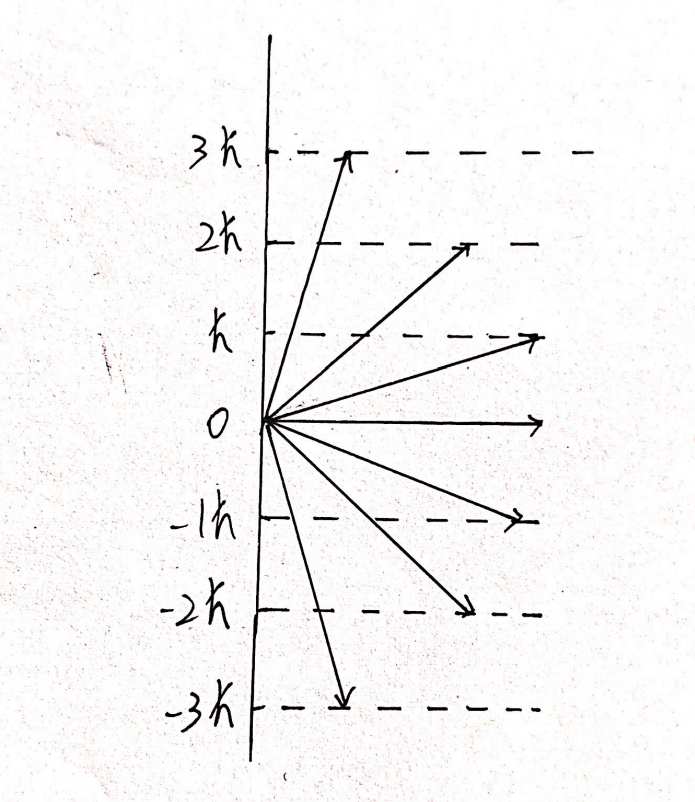
\includegraphics[scale=0.5]{P1.png}
    \caption{Projection of $L$ on the z-axis}
\end{figure}
\section{Problem 3}
    \noindent(a)$\mu=\frac{m^2}{2m}=\frac{m}{2}$
    \\$I=\mu(2a)^2=2ma^2$
    \\$\hat{H}\psi=\frac{\hat{L}^2}{2I}\psi=E\psi\rightarrow\hat{L}^2\psi=4Ema^2\psi$
    \\Since $L=\hbar\sqrt{l(l+1)}$
    \\$E_l=\frac{\hbar^2l(l+1)}{4ma^2}$
    \\$[-\frac{\hbar^2}{2\mu}\frac{\partial}{\partial r}(r^2\frac{\partial}{\partial r})+\frac{\hat{L}}{2\mu r^2}+V(r)]\psi=E\psi$
    \\$[-\frac{\hbar^2}{2\mu}\frac{\partial}{\partial r}(r^2\frac{\partial}{\partial r})+\frac{\hbar^2l(l+1)}{2\mu r^2}+V(r)]R(r)=ER(r)$
    \\Then $E=-\frac{E_1}{n^2}$ where $E_1=\frac{\mu e^4}{32\pi^2\hbar^2\epsilon_0}=\frac{me^4}{64\pi^2\hbar^2\epsilon_0}$ and $R_{nl}=Ae^{-\frac{r}{a_0n}r^lL_{nl}(\frac{r}{a_0})}$
    \\(b)\begin{figure}[H]
        \centering
        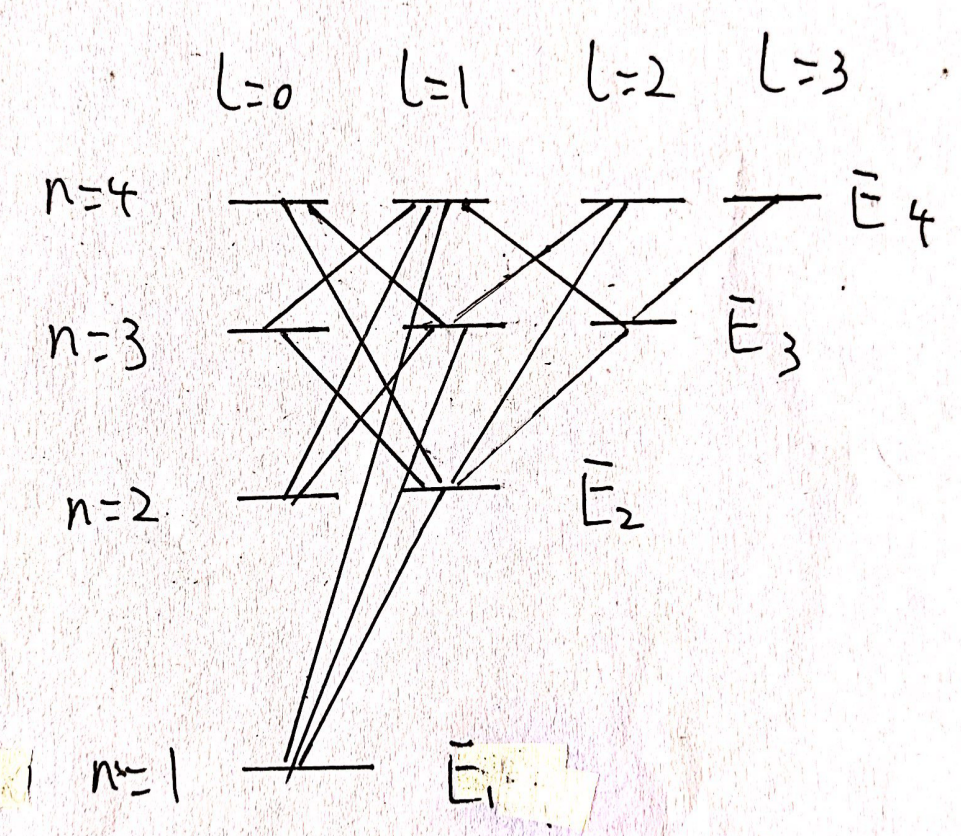
\includegraphics[scale=0.25]{P2.png}
        \caption{Energy level diagram}
    \end{figure}
    \noindent For transition energy $E_1=\frac{\hbar^2(l+1)}{2I}=\frac{\hbar^2(1+1)}{2I}=\frac{\hbar^2}{I}$
    \\$\bigtriangleup E=E_{l+1}-E_l=\frac{\hbar^2(l+2)(l+1)}{2I}-\frac{\hbar^2l(l+1)}{2I}=\frac{2\hbar^2(l+1)}{2I}=(l+1)\frac{\hbar^2}{I}$
    \\Hence $E_n=nE_1$ where $n=1,2,3\cdots$
    \\(c) $I=2ma^2=2\cdot1.67\cdot10^{-27}\cdot(3.7\cdot10^{-11})^2=4.57\cdot10^{-48}$
    \\$E_1=\frac{\hbar^2}{2ma^2}=\frac{\hbar^2}{I}=2.41\times10^{-21}$J
    \\(d) $\bigtriangleup E_{l\rightarrow l+1}=\frac{2\hbar^2(l+1)}{4ma^2}$
    \\Hence when $l=0$ we have the lowest transition energy $\bigtriangleup E_{l\rightarrow l+1}=\frac{\hbar^2}{2ma^2}=0.015$eV
    \\$\bigtriangleup E=\frac{hc}{\lambda}\rightarrow\lambda=\frac{hc}{\bigtriangleup E}=\frac{6.63\cdot10^{-34}3\cdot10^8}{2.41\times10^{-21}}=8.25\cdot10^{-5}m$
    \\It's in the visible light region close to Paschen region.
\section{Problem 4}
\noindent (a)$L=r\times p$, since $r$ and $p$ are perpendicular to each other in the xy-plane, then $L$ is along the z-axis, hence it has two zero components
\\According to classic mechanic, for the total energy, since $V(x)=0,E=K=\frac{1}{2}I\omega^2=\frac{L^2}{2I}$
\\(b) $\hat{H}=\frac{\hat{L_z}^2}{2I}+V=-\frac{\hbar^2}{2I}\frac{\partial^2}{\partial\varphi^2}+V$
\\Since $V=0,-\frac{\hbar^2}{2I}\frac{\partial^2\psi}{\partial\varphi^2}=E\psi\rightarrow-\frac{\hbar^2}{2I}\frac{\partial^2\phi(\varphi)}{\partial\varphi^2}=E\phi(\varphi)\rightarrow \phi=Ce^{\pm\sqrt{-\frac{2IE}{\hbar^2}}\varphi}, E$ can be any real number
\\Hence $\psi=Ce^{\pm\sqrt{-\frac{2IE}{\hbar^2}}\varphi}$
\\ (c) $\psi(\varphi+2\pi)=\psi(\varphi)\rightarrow\int_0^{2\pi}C^2\cos^4(\varphi)d\varphi=1\rightarrow C^2\frac{3\pi}{4}=1\rightarrow C=\pm\frac{2}{\sqrt{3\pi}}$
\section{Problem 5}
\noindent (a) $n=6,l=3$
\\ (b) $E_6=-\frac{E}{n^2}=-\frac{13.6}{36}=0.38$eV
\\ (c) $|L|=\sqrt{L^2}=\sqrt{3(3+1)\hbar^2}=2.3\times10^{-33}$
\\ (d) $L_z=m\hbar=\pm1.989\times10^{-33},\pm1.326\times10^{-33},\pm6.63\times10^{-34},0$
\section{Problem 6}
\noindent (a)$\psi_{210}=\frac{1}{4\sqrt{2\pi}}(\frac{Z}{a_0})^{3/2}\frac{Zr}{a_0}e^{-Zr/2a_0}\cos\theta$
\\Since it's hydrogen atom, $Z=1,\psi_{210}=\frac{1}{4\sqrt{2\pi}}(\frac{1}{a_0})^{3/2}\frac{r}{a_0}e^{-r/2a_0}\cos\theta$
\\$P(r)=\psi_{210}^*\psi_{210}4\pi r^2=\frac{r^4}{8a_0^5}e^{-r/a_0}\cos^2\theta,$ hence $P(r)\propto r^4e^{-r/a_0}$
\\(b) $\frac{\mathrm{d}P(r)}{\mathrm{r}}=\frac{r^3}{2a_0^5}e^{-r/a_0}\cos^2\theta-\frac{1}{a0}\frac{r^4}{8a_0^5}e^{-r/a_0}\cos^2\theta=0$
\\ $r=4a_0\text{ or }r=0$
\section{Problem 7}
\noindent $\psi_{000}=\frac{1}{\sqrt{\pi}}(\frac{Z}{a_0})^{3/2}e^{-Zr/a_0}$
\\Since $Z=1$, then $P(r)=4r^2\frac{1}{a_0^3}e^{-2r/a_0}$
\\Since $a_0=5.29\cdot10^{-11}>>R_0=10^{-15},e^{-2r/a_0}\approx0$
\\$\int_0^{R_0}P(r)\mathrm{d}r=\int_0^{10^{-15}}4r^2\frac{1}{a_0^3}\mathrm{d}r=9\cdot10^{-15}$
\section{Problem 8}
\noindent $I=\frac{2}{5}mR^2=\frac{2}{5}9.1\cdot10^{-31}(10^{-15})^2\approx3.64\cdot10^{-60}$
\\$\omega=\frac{|L|}{I}=\frac{|S|}{I}=\frac{\hbar\sqrt{\frac{3}{4}}}{3.64\cdot10^{-60}}\approx2.5\cdot10^{25}$rad/s
\\$v=\omega R=2.5\cdot10^{25}10^{-15}=2.5\cdot10^{10}$m/s
\\The speed is larger than the speed of light, hence the result from classic mechanic is incorrect.
\section{Problem 9}
\noindent (a) We should expect to see 4 lines with $j=\pm\frac{3}{2}$ because $l=0,s=\frac{3}{2}$
\\Hence the lines corresponds $m_s=\pm\frac{3}{2},\pm\frac{1}{2}$
\\ (b) We should expect to see 3 lines with $m=\pm1,0$ 
\section{Problem 10}
\noindent $\textbf{L}=\hbar\sqrt{l(l+1)}=1.05\cdot10^{-34}\sqrt{2\cdot3}\approx2.58\cdot10^{-34}\text{N}\cdot\text{m}\cdot\text{s}$
\\$j=l\pm\frac{1}{2}=\frac{5}{2}\text{ or }\frac{3}{2}$
\\The corresponding $\textbf{J}\approx3.11\cdot10^{-34}\text{ or }2.03\cdot10^{-34}\text{N}\cdot\text{m}\cdot\text{s}$   
\end{document}